Before starting to analyze the structures, let us first have an overview of how MEMS microphones are made and what are the advantages of using them. \\
MEMS microphones are acoustic-to-electrical transducers that convert sound waves into electrical signals using microelectromechanical systems technology. \\
Compared to conventional microphones, MEMS microphones offer several advantages such as compact size and high integration capability with electronic circuits. \\
These features make them particularly suitable for miniaturized devices. \\
A MEMS microphone is composed of two principal parts:

\begin{itemize}
    \item \textbf{Diaphragm}: It is a membrane that is free to move under external pressure.
    \item \textbf{Backplate}: It is the static part, used to support and position the diaphragm.
\end{itemize}

\noindent
The membrane and the backplate are mounted one over the other, as shown in \autoref{fig:MEMS_microphone_structure}.

\vspace{0.5cm}
\begin{figure}[h!]
    \centering
    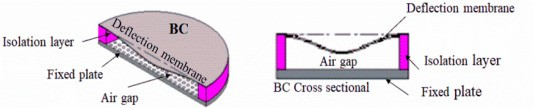
\includegraphics[width=1\linewidth]{img/MEMS_microphone_structure.jpg}
    \caption{MEMS microphone structure}
    \label{fig:MEMS_microphone_structure}
\end{figure}
\vspace{0.5cm}

\noindent
The goal is to detect pressure variations acting on the diaphragm. \\
To achieve this, two electrodes are connected to the structure in order to measure the variation in electrical capacitance between the diaphragm and the bottom plate. \\
The problem with the common structure shown above is that the air gap between the membrane and the bottom plate has a non-negligible viscosity, which can compromise the functionality of the microphone. \\
Air viscosity, in fact, modifies the ideal relationship that links pressure to the capacitance variation of the membrane. \\
The two structures considered are taken from the paper \cite{krishnapriya2014} and employ common strategies to reduce the effect of air viscosity in the gap. \\
The idea is to introduce holes either in the diaphragm or in the bottom plate to allow air to pass through them.